 \documentclass[oneside,a4paper,12pt]{pictreport}
\usepackage{dirtree}
\usepackage{enumitem}
\usepackage{amsmath}
\usepackage{listings}
%\usepackage[table,xcdraw]{xcolor}
\usepackage{graphicx}
\usepackage{multirow}
\usepackage{enumitem}
\setlist[enumerate]{itemsep=0mm}


\lstset{basicstyle=\ttfamily,
  showstringspaces=false,
  commentstyle=\color{red},
  keywordstyle=\color{blue}
}
%\usepackage{showframe}
%\hoffset = 8.9436619718309859154929577464789pt
%\voffset = 13.028169014084507042253521126761pt
\usepackage{enumitem}
\setlist{parsep=0pt,listparindent=\parindent} %


\fancypagestyle{plain}{%
  \fancyhf{}
  \fancyfoot[C]{PICT, Department of Computer Engineering, 2017}
  \fancyfoot[R]{\thepage}
}
\pagestyle{fancy}
\fancyhead{}
\renewcommand{\headrulewidth}{0pt}
\footskip = 0.625in
\cfoot{}
\rfoot{}

\usepackage[hidelinks]{hyperref}
\usepackage{tikz}
\usetikzlibrary{arrows,shapes,snakes,automata,backgrounds,petri}

\usepackage{tabularx}

\usepackage[nottoc,notlot,notlof,numbib]{tocbibind}
\usepackage[titletoc]{appendix}
\usepackage{titletoc}
\renewcommand{\appendixname}{Annexure}
\renewcommand{\bibname}{REFERENCES}

\setcounter{secnumdepth}{5}
\usepackage{float}
\usepackage{subcaption}
\usepackage{multirow}

\usepackage[ruled,vlined]{algorithm2e}

\begin{document}

\picttitlepage{SENTIMENT ANALYSIS USING ORIGINAL AND REVERSED REVIEWS}{Kaushik S. Hande}{}{Prof. A. G. Phakatkar}

%\companycertificate{BEHAVIORAL ASSESSMENT OF INTERNAL AND EXTERNAL CANDIDATES OF MULTIPLE ORGANIZATIONS USING SENTIMENT ANALYSIS AND EMOTION MINING}{Sagar S. Patil}{}{Mr. Vijay Kumbhar}{Mr. Vijay Kumbhar}{}

\pictcertificate{SENTIMENT ANALYSIS USING ORIGINAL AND REVERSED REVIEWS}{Kaushik S. Hande}{}{Prof. A. G. Phakatkar}{}





\setcounter{page}{0}
\frontmatter
\cfoot{PICT, Department of Computer Engineering, 2017}
\rfoot{\thepage}
\pagenumbering{Roman}
\pictack{SENTIMENT ANALYSIS USING ORIGINAL AND REVERSED REVIEWS}{Kaushik S. Hande}{}{}

\listoffigures 
\listoftables
		
\begin{pictabstract}
Human Computer Interaction(HCI) is an active focus of research. Considering the motivation, need and challenges, we are proposing fingertip detection system with vision approach for Desktop handling operation.

The advantages of such system will be to avoid physical devices such as keyboard, mouse etc.
\end{pictabstract}



% \maketitle
\tableofcontents
\mainmatter



\titleformat{\chapter}[display]
{\fontsize{16}{15}\filcenter}
{\vspace*{\fill} \bfseries\LARGE\MakeUppercase{\chaptertitlename}~\thechapter}
{1pc}
{\bfseries\LARGE\MakeUppercase}
[\thispagestyle{empty}\vspace*{\fill}\newpage]





\setlength{\parindent}{11mm}
\chapter{SYNOPSIS}


\section{Dissertation Title}
SENTIMENT ANALYSIS USING ORIGINAL AND REVERSED REVIEWS

%\section{Sponsorship}
%Webonise Lab, Pune.

%\section{External Guide} 
%Mr. Vijay Kumbhar

\section{Internal Guide}
Prof. A. G. Phakatkar



\section{Problem Statement}
\label{sec:problem_def}
``To develop Vision based Human Computer Interaction System using Fingertip Tracking for Desktop Handling operation.''

\section{Objectives}
\begin{itemize}
    \item Design and implement fingertip detection algorithm. 
    \item Design and implement fingertip tracking algorithm. 
    \item Design and implement virtual keyboard. 
    \item Execute Windows API for execution. 
    \item Test and analyze the system. 
    \item 
    \item 
    \item 
\end{itemize}

\section{Hypothesis}

Vision based Hand detection and tracking can determine cursor movements using operating system's system calls. Gestures determined by using computer vision techniques can be utilized to generate callback functions to implement various system functions. CamShift algorithm with Kalman filter can be used to determine accurate and exact location of cursor to give better Human Computer Interaction using virtual keyboard with web-cam.

\section{Relevant Mathematics Associated with Dissertation}

\subsection{Mathematical Model}
$S=\{s,e,I,F,F_{s},F_{t},F_{f},O|\phi\}$\\\\
%\end{equation*}
where,\\
s = start state\\
e = end state\\
F = Feature Vector for G\\
G = set of Gestures\\
$F_{s} =$ Fingertip detection function\\
$F_{t} =$ Fingertip tracking function\\
$F_{f} =$ Feature Extraction and Matching function\\
I = set of Inputs\\
I = \{M,G\}\\\\
where,\\
M = \{RC,LC,MC..Drag\}\\
RC = Right Click\\
LC = Left Click\\
MC = Middle Click\\
G = \{VK,M,SG\}\\\\
where\\
VK = Virtual Keyboard System\\
$SG = \{VK_{0},VK_{1},RCG,LCG,MCG,DragG,G1..G10\}$\\
where
SG  = Special Gestures\\
$VK_{0} =$ Virtual Keyboard off\\
$VK_{1} =$ Virtual Keyboard on\\
RCG = Right Click Gesture\\
LCG = Left Click Gesture\\

F = \{KS,MS,GF\}\\\\
where\\
KS = System Keyboard functions mapped to K\\
MS = System mouse functions mapped to M\\
GF = Gesture functions mapped to G\\
O = Output \\
O = \{KSe,MSe,GFe,EMd\}\\\\
where\\
KSe = API execution of Keyboard\\
MSe = API execution of Mouse\\
GFe = API execution of Gesture Functions\\
EMd = Display of Error Messages\\

Success: If $I_{i} = F_{j},1<i<=|I|,1<j<=|F| Then Execute O_{i}$\\
Failure: Else No Execution (or print Error Messages)\\


\subsection{Metrics for Performance Evaluation}
Several statistical measures are used for performance evaluation - 
\begin{itemize}
\item Accuracy-is the proximity of measurement results to the true value.
\begin{equation}
\frac{TP + TN}{TP + TN + FP + FN}
\end{equation}
\item Sensitivity- measures the proportion of positives that are correctly identified
\begin{equation}
\frac{TP}{TP + FN}
\end{equation}
\item Specificity- measures the proportion of negatives that are correctly identified 
\begin{equation}
\frac{TN}{TN + FP}
\end{equation}
\item Positive predictive value- are the proportions of positive results in statistics and diagnostic tests 
\begin{equation}
\frac{TP}{TP + FP}
\end{equation}
\item Negative predictive value- are the proportions of negative results in statistics and diagnostic tests 
\begin{equation}
\frac{TN}{TN + FN}
\end{equation}
\end{itemize}

\chapter{TECHNICAL KEYWORDS}
\section{Area of Dissertation}
Computer Vision, Human Computer Interaction, Fingertip detection, Hand tracking and Segmentation, Hand Gesture Recognition.

\section{ACM Keywords}
\begin{enumerate}[label=\Alph*]
    \item Information Systems
    \begin{enumerate}[label*=.\arabic*]
        \item Retrieval tasks and goals
        \begin{enumerate}[label*=.\arabic*]
            \item Sentiment analysis
            \item Clustering and classification
        \end{enumerate}
    \end{enumerate}
    \item Information storage systems
        \begin{enumerate}[label*=.\arabic*]
            \item Storage architectures
            \begin{enumerate}[label*=.\arabic*]
                \item Distributed storage
            \end{enumerate} 
        \end{enumerate}
    \item Information systems applications 
        \begin{enumerate}[label*=.\arabic*]
            \item Data Mining
            \begin{enumerate}[label*=.\arabic*]
                \item Emotion Mining
            \end{enumerate}
        \end{enumerate}
    \item Computing methodologies
        \begin{enumerate}[label*=.\arabic*]
            \item Parallel computing methodologies
            \item Machine learning
            \begin{enumerate}[label*=.\arabic*]
                \item Supervised learning by classification
                \begin{enumerate}[label*=.\arabic*]
                    \item Multinomial Naive Bayes
                    \item Random Forest
                    \item Support Vector Machines
                \end{enumerate}
            \end{enumerate}
        \end{enumerate}
    \item Security and privacy
    \begin{enumerate}[label*=.\arabic*]
        \item Cryptography
        \begin{enumerate}[label*=.\arabic*]
            \item Kerberos Authentication Protocol
        \end{enumerate}
    \end{enumerate}
\end{enumerate}
\chapter{INTRODUCTION}

\section{Dissertation Idea}

\hspace{1.1cm} Today's organizations assess their external candidates, candidates they want to recruit and internal candidates or employees currently working, based on their compatibility to organization's culture and fitness in role associated to them. They use multiple tests that consists of several roles scenarios as well as capability questions for assessment. Assessing candidate’s behavior is equally important to determine mindset and thoughts to recent and trending topics. This can be done in two ways:

\begin{itemize}
\item Behavioral assessment test that comprises of some questions that is used to observe, describe and predict candidate’s behavior.
\item Building a iterative behavioral profile by analyzing candidate’s profile on social media sites, their reaction to recent trending topics. Reactions can be mapped to emotion classes, which then give a more precise in-depth understanding of candidate’s behavior.
\end{itemize}
Assessment results along with inclusion of behavioral profiling of candidates is recorded by HR. This helps organizations in forming proper structure, planning, management, allocation of candidate to proper product development and operational efficiency.\\\\
Predictive analytics combined with proposed behavioral model gives organization essential information regarding internal candidates and helps in making key decisions like customized employment value proposition. Tweets from Twitter of candidates are collected, that becomes our input dataset for a particular candidate. Dataset persists in HDFS, thus provides information availability even if one of the connected node goes down. Only selective data from dataset is brought down to Alluxio, virtual distributed storage system. \\\\
Alluxio storage system stores in-memory data, so only limited data can be stored in the storage system. Therefore, Alluxio makes use of a optimized allocators and evictors like Max Free Allocator or Greedy Allocator to move data between memory and underFS storage layer like HDFS. Candidate is classified to emotion classes based on sentiment analysis’s results. We can see difference in the behavior of candidates as we are analyzing social media profile by month’s usage. t helps organizations to see patterns in behavior of candidate.\\\\
Our proposed model uses Naive Bayes Classifier for classification. Classifier's execution occurs as a Spark job which runs distributively on several connected commodity hardware configured nodes. Hadoop and Spark does not provide any authentication among its components while running spark job. Therefore, it is necessary to provide mutual authentication among server nodes, Hadoop components - Domain specific as well as infrastructure components. Mutual authentication is achieved by integrating Kerberos into Hadoop, Spark and Alluxio.
\section{Motivation of Dissertation}

\hspace{1.1cm} In various organizations, candidates are assessed for criteria of suitability to organization’s culture and their specific role. Behavior of a candidate plays a vital role in progress of organization. A candidate may excel at his role but do not have proper attitude towards his teammates, may degrade the quality and productivity of his entire team. Candidate may lie in behavioral assessment test but they do not hide their reactions on social media sites about current trending topics like political, scientific etc. By collecting those reactions, we can construct behavioral model of candidates and can predict future behavior.
 

\chapter{LITERATURE SURVEY}

We studied the following related systems to discover their advantages, drawbacks and limitations and these are discussed below.

\section{Affective Text Mining}
\hspace{1.1cm}Previous work focused on mining affective content from text documents using sentiment classification. However, study does not explores extraction of social emotions from multiple social media sites and building a behavioral profile of a candidate that quicksilver with consideration of new posts to sites. The most related direction to work is emotion prediction and classification. Affective text aims to add notes giving explanation to predefined list of emotions and/or polarity orientation (positive, negative and neutral). Alm et al [1] explored text-based emotion prediction using supervised learning approaches. Strapparava and Mihalcea [2] evaluated methods for the automatic identification of six emotions. Tokuhisa et al [3] proposed a two step model for emotion classification using emotion-provoking event instances. Yang et al [4] investigated the emotion classification of blogs using machine learning techniques.

\section{Emotion Term Model}
A method to model the word-emotion associations is emotion-term model [14], which uses Naive Bayes with the assumption that words are independently generated from social emotion labels. The model needs to be extended to account not only social emotion labels but querying entire text to generate more precise emotion-term relationship. Emotion-term model generates each word \textit{$w_i$} of document \textit{d} in two sampling steps.
\begin{itemize}
\item sample emotion \textit{$e_i$} according to the emotion frequency count
\item sample a word \textit{$w_i$} given the emotion under the conditional probability P($w|e$)
\end{itemize}
\par The model parameters can be learned by maximum-likelihood estimation. In particular, the conditional probability of a word \textit{w} given an emotion \textit{e} can be estimated as follows:
\begin{equation}
P(w|e) = \frac{|(w, e)|}{\sum|(w, e)|} 
\end{equation}
\par where $w^i \epsilon  W$, $|(w, e)|$ is the co-occurrence count between $w \epsilon W$ and emotion $e \epsilon E$ for all documents. It is formally derived based on the word and emotion frequency counts
\begin{equation}
|(w, e)| = S + \sum\limits_{d \epsilon D} \delta_{d,w} . \Upsilon_{d,e}
\end{equation}
\par where S is a small smoothing constant that is set to 1. For predicting emotion on a new document \textit{b}, Bayes theorem can be applied under the term independence assumption
\begin{equation}
P(e|d) = \frac{P(d|e)P(e)}{P(d)} \alpha P(d|e)P(e)
\end{equation}
\par where P(e) is the a priori probability of emotion e. It can again be calculated by maximum likelihood estimation from the emotion distribution of the entire collection.

\section{Authentication Methods For Hadoop}
\hspace{1.1cm}Multiple clients submit their MapReduce jobs for processing. Before submitting any jobs, a client needs to get authenticated by Authentication Server. Somu et al [5] provides a method which is symmetric key based. It uses single authentication factor, supports only gate-level authentication and has more communication overheads. Rubika method of authentication [6] is also designed to support client authentication only. Wei et al [7] ensures the authenticity of messages sent from one MR-job component to another. There is need of mutual authentication between MR components and MR infrastructure components. J. Zhao et al [8] supports the authentication of a client to MR application and authentication between pair of domain specific MR components.


\section{Gap Identification Through Literature Survey}

The following table shows the literature survey about different techniques of analyzing sentiment from social media text and emotion classification.

\renewcommand{\arraystretch}{1.0}
\begin{center}
\begin{table}[h!]
\caption{Literature Survey} 
\begin{tabular}{|l|l|l|l|}
\hline
No. & Reference                                                              & Techniques                                                                & Description                                                                 \\
\hline
1   & \begin{tabular}[c]{@{}l@{}}Hand Detection\\ Techniques to hand \\gesture Recognition for\\ Natural Human \\Computer Interaction\end{tabular}                                                             & \begin{tabular}[c]{@{}l@{}}Hand Detection using \\ Lab Color Space \\       and\\ Mean Shift Algorithm \end{tabular}                                                                    & \begin{tabular}[c]{@{}l@{}}Better results on \\ skin color detection using \\ HTS algorithm streams.\end{tabular}                                                                                                                                                                                         \\
\hline
2   & \begin{tabular}[c]{@{}l@{}}Hand Gesture Recognition \\for Indian Sign Language\end{tabular}                                                           & \begin{tabular}[c]{@{}l@{}}HSV color model \\and General Camshift\\ algorithm\end{tabular}                                  & \begin{tabular}[c]{@{}l@{}}The Gesture Recognition \\System takes the input \\hand gestures through \\ in-built web camera.\end{tabular}                                                                                                                                                                      \\
\hline
3   & \begin{tabular}[c]{@{}l@{}}A Novel Projector-Camera \\Interaction System \\with the Fingertip\end{tabular}                 & \begin{tabular}[c]{@{}l@{}}Prediction
Method and \\triangulation Zhang's\\ method \end{tabular}            & \begin{tabular}[c]{@{}l@{}}Projector and binocular \\vision system based on \\two cameras is applied \\for detecting the depth\\ of fingertips and \\touch operation.\end{tabular}                                                                                                                                                          \\
\hline
4   & \begin{tabular}[c]{@{}l@{}}Hand gesture based \\user interface for \\computer using a camera \\and Projector\end{tabular}                                          & \begin{tabular}[c]{@{}l@{}} The YCrCb color space \\with single Gaussian\\ and Camshift tracking \\algorithm\end{tabular}                                                         & \begin{tabular}[c]{@{}l@{}}A hand gesture based \\human computer \\interaction system \\comprising of a \\webcam and a \\pocket projector.\end{tabular}                                                                                                                                                                                        \\
\hline
5   & \begin{tabular}[c]{@{}l@{}}Real-Time Robust Hand \\Tracking Based on \\Camshift and Motion \\Velocity\end{tabular} & \begin{tabular}[c]{@{}l@{}} Improved Camshift \\algorithm \\with KLT tracking. \end{tabular}  & \begin{tabular}[c]{@{}l@{}} Probability of Bayesian\\ skin color is used \\to refine the velocity \\of hand motion.\end{tabular}                                                                                                                                                 \\
\hline
6   & \begin{tabular}[c]{@{}l@{}}Gesture Recognition in \\Ego-Centric Videos \\using Dense Trajectories \\and Hand Segmentation\end{tabular}                                                                                    & \begin{tabular}[c]{@{}l@{}} Dense trajectories\\
extracted \\around hand regions\end{tabular}                                                           & \begin{tabular}[c]{@{}l@{}}Dense features are\\ extracted around regions\\ selected by a new hand \\segmentation technique.\end{tabular}                                                                                                                                                                          \\
\hline

7  & \begin{tabular}[c]{@{}l@{}}A 3D Hand Tracking\\ Design for Gesture\\ Control in Complex \\Environments\end{tabular}                                                                                & \begin{tabular}[c]{@{}l@{}}3D hand tracking design\end{tabular}                         & \begin{tabular}[c]{@{}l@{}}It segments hands \\out of entire image \\and also facilitates \\depth estimation of \\tracked hands in\\ real-time by dual \\camera systems.\end{tabular}                                                                                                                                                                      \\
\hline
8  & \begin{tabular}[c]{@{}l@{}}Hand tracking and \\Gesture Recognition\end{tabular}                                                                              & \begin{tabular}[c]{@{}l@{}}Kalman filter and\\
derived Scale Invariant \\Feature Transform (SIFT).\end{tabular}                  & \begin{tabular}[c]{@{}l@{}}It presents a method \\for tracking and \\recognizing hand\\ gestures by extracting \\ unique invariant \\features from gestures.\end{tabular}  \\          
\hline
\end{tabular}
\end{table}
\end{center}
\newpage
\renewcommand{\arraystretch}{1.0}
\begin{center}
\begin{table}[h!]
\begin{tabular}{|l|l|l|l|}
\hline
No. & Reference                                                              & Techniques                                                                & Description                                                                 \\
\hline
9  & \begin{tabular}[c]{@{}l@{}}Hand Position Tracking \\Using a Depth Image \\from a RGB-d Camera\end{tabular}                                               & \begin{tabular}[c]{@{}l@{}}RGB image based on \\the skin color
Hand \\Tracking \end{tabular}                                                      & \begin{tabular}[c]{@{}l@{}}The algorithms can be\\ used for natural user \\interfaces, the guidance of the\\end effector \\of an industrial robot\\ and hand segmentation.\end{tabular}
\\    
\hline
10 & \begin{tabular}[c]{@{}l@{}}Indian Sign Language \\Recognition: \\Database Creation, Hand \\Tracking and Segmentation\end{tabular}                       & \begin{tabular}[c]{@{}l@{}}YcbCr based skin \\color model \end{tabular}     & \begin{tabular}[c]{@{}l@{}}This algorithm works \\on motion tracking, \\edge detection and \\skin color detection.\end{tabular}          \\
\hline
\end{tabular}
\caption{Literature Survey} 
\end{table}
\end{center}

\chapter{PROBLEM DEFINITION AND SCOPE}

\section{Goals}
\begin{itemize}
\item Understanding of existing Cultural Framework and Role Scenarios.
\item Designing a web platform that carries out functionality of the system.
\item Understanding of Storage File Systems – Apache's HDFS and Alluxio.
\item Integrating Alluxio with Apache's HDFS and Apache's Spark.
\item Understanding Sentiment Analysis and Emotion Mining Approaches.
\item Classifying candidate's documents into emotion categories.
\end{itemize}

\section{Objectives}

Please refer Chapter 1, Section 1.7 on Page XX

\section{Statement of Scope}
\begin{itemize}
\item Analyzing candidate's tweets distributively on multiple node Spark cluster.
\item Classify candidate's tweets into seven emotion categories and three polarities.
\item Integrating Alluxio core services with Apache HDFS and Apache Spark.
\item Validates candidate's emotion classification.
\item Validates candidates comparison by emotion categories. 
\end{itemize}

\section{Software Context}
\subsection{Apache Spark} 
Spark [9] provides fast cluster computing system. It's high level APIs in Java, Python, Scala, Python and R are used. It also uses Hadoop client's libraries for performing operation on data stored in HDFS. Spark system in cluster mode is deployed to take advantage of commodity hardware by using Hadoop YARN as cluster manager. Spark with Mahout APIs can be used for calculating term frequencies, generating TFIDF vectors, writing and reading from HDFS and Alluxio and classification. By using Spark, more records in less time is classified efficiently.

\subsection{Apache Hadoop}
Hadoop's HDFS [10] stores huge amount of training data in HDFS for distributed processing. Mahout APIs can access data stored in HDFS for processing. It provides scalable environment and fault-tolerant file systems.

\subsection{Alluxio}
It provides memory centric design and unified name space for different storage system. Alluxio [11] improves processing speed for big data applications while providing a common interface of data access. Haoyuan Li et al. [12] explains how Alluxio speeds up read and write throughput. 

\subsection{Kerberos}
To provide a level of security among Hadoop components like Resource Manager etc. Kerberos [13] sets up a Key Distribution Center. KDC has three main components. Kerberos Database which stores users and services identity. Authentication server resides as a separate physical server. It issues tickets upon initial request. Ticket Granting Service responsible for providing service tickets. By using these three components, communication is secured between core components of Alluxio, Spark and Hadoop.

\subsection{Laravel PHP}
A PHP framework that provides useful tools to securely built a web application with an ease. It provides authentication, amazing ORM, painless routing and powerful queue library.

\chapter{DISSERTATION PLAN}

\section{Purpose of the Document}
This document specifies and estimates various risks associated with this project and states how they are handled. It also states the project plan in terms of task and their dependency.

\section{Technical Constraints}
\begin{itemize}
\item To build a classification module that distributes data and execution among spark executors.
\item To fetch candidate's tweets in a CSV format and store it in Alluxio.
\end{itemize}

\section{Dissertation Estimates}
\subsection{Reconciled Estimates}
\subsubsection{Cost Estimates}
No cost is required for tools and software as open source softwares are used.
\subsubsection{Time Estimates}
Calendar time required: 11 months.
\subsubsection{Dissertation Resources}
\begin{itemize}
\item People : Single Person
\item Hardware resources used are mentioned in Chapter 6, Section 6.5 on Page XX
\item Software resources used are mentioned in Chapter 6, Section 6.6 on Page XX
\end{itemize}

\section{Risk Management}
This section discusses dissertation risks and the approach to managing them.
\subsection{Risk Identification}
For risks identification, review of scope document, requirement specifications and schedule is done. Answers to questionnaire revealed some risks. Following risk identification questionnaire has been referred.
\begin{itemize}
\item Are requirements fully understood by the software engineering team and its customers?
\item Have customers been involved fully in the definition of requirements?
\item Do end-users have realistic expectations?
\item Does the software engineering team have the right mix of skills?
\item Are project requirements stable?
\item Is the number of people on the project team adequate to do the job?
\item Do all customer/user constituencies agree on the importance of the project and on the requirements for the system/product to be built?
\end{itemize}

\subsection{Risk Analysis}
The risks for the dissertation are analyzed within the constraints of time and quality. Risk can be as follows:

\begin{itemize}
\item Out of memory error, when training Naive Bayes Model.
\item Spark executors were getting lost.
\item Incorrect candidate results.
\end{itemize}
Please refer Table 5.1, 5.2 and 5.3 for detail description.

\renewcommand{\arraystretch}{1.5}
\begin{table}[h!]
\caption{Risk Table}
\begin{tabular}{|l|l|l|l|l|l|}
\hline
\textbf{ID} & \textbf{Risk Description} & \textbf{Probability} & \multicolumn{3}{c|}{\textbf{Impact}}                                         \\ \hline
            & \textbf{}                 & \textbf{}            & \textbf{Schedule} & \textbf{Quality} & \textbf{Overall} \\ \hline
1           & Out of Memory             & Low                  & Low                      & High                    & High                    \\ \hline
2           & Executors Lost            & Medium               & Medium                   & High                    & Medium                  \\ \hline
3           & Incorrect Results         & Medium               & Medium                   & High                    & High                    \\ \hline
\end{tabular}
\end{table}

\begin{table}[h!]
\centering
\caption{Risk Probability Definitions}
\begin{tabular}{|l|l|l|}
\hline
\textbf{Probability} & \textbf{Value}                   & \textbf{Description} \\ \hline
High                 & Probability of the occurrence is & \textgreater 75\%    \\ \hline
Medium               & Probability of the occurrence is & 26\% - 74\%          \\ \hline
Low                  & Probability of the occurrence is & 25\%                 \\ \hline
\end{tabular}
\end{table}

\begin{table}[h!]
\centering
\caption{Risk Impact Definitions}
\begin{tabular}{|l|l|l|}
\hline
\textbf{Impact} & \textbf{Value}    & \textbf{Description}                                                                                                                                        \\ \hline
Very High       & \textgreater 10\% & Schedule impact or Unacceptable quality                                                                                                                     \\ \hline
High            & 5\%-10\%          & Schedule impact or Some parts of the project have low quality                                                                                               \\ \hline
Low             & \textless5\%      & \begin{tabular}[c]{@{}l@{}}Schedule impact or Barely noticeable degradation in quality\\ Low Impact on schedule or Quality can be incorporated\end{tabular} \\ \hline
\end{tabular}
\end{table}

\subsection{Overview of Risk Mitigation, Monitoring and Management}
Please refer Table 5.4, 5.5 and 5.6 for detail description.

\begin{table}[h!]
\centering
\caption{Risk 1}
\label{my-label}
\begin{tabular}{|l|l|}
\hline
\textbf{Risk ID}          & 1                                                    \\ \hline
\textbf{Risk Description} & Out of memory error, when training Naive Bayes Model \\ \hline
\textbf{Category}         & Configuration                                        \\ \hline
\textbf{Source}           & Software Requirement Specification Document          \\ \hline
\textbf{Probability}      & Low                                                  \\ \hline
\textbf{Impact}           & High                                                 \\ \hline
\textbf{Response}         & Mitigate                                             \\ \hline
\textbf{Strategy}         & Changing number of features resolves this issue.     \\ \hline
\textbf{Risk Status}      & Occurred and Resolved                                \\ \hline
\end{tabular}
\end{table}


\begin{table}[h!]
\centering
\caption{Risk 2}
\label{my-label}
\begin{tabular}{|l|l|}
\hline
\textbf{Risk ID}          & 2                                                                     \\ \hline
\textbf{Risk Description} & Spark executors were getting lost                                     \\ \hline
\textbf{Category}         & Configuration                                                         \\ \hline
\textbf{Source}           & Software Requirement Specification Document                           \\ \hline
\textbf{Probability}      & Medium                                                                \\ \hline
\textbf{Impact}           & Medium                                                                \\ \hline
\textbf{Response}         & Mitigate                                                              \\ \hline
\textbf{Strategy}         & Increasing heart beat interval and network timeout resolve this issue \\ \hline
\textbf{Risk Status}      & Occurred and Resolved                                                 \\ \hline
\end{tabular}
\end{table}
\begin{table}[h!]
\centering
\caption{Risk 3}
\label{my-label}
\begin{tabular}{|l|l|}
\hline
\textbf{Risk ID}          & 3                                           \\ \hline
\textbf{Risk Description} & Incorrect Candidate Results                 \\ \hline
\textbf{Category}         & Development Environment                     \\ \hline
\textbf{Source}           & Software Requirement Specification Document \\ \hline
\textbf{Probability}      & Medium                                      \\ \hline
\textbf{Impact}           & High                                        \\ \hline
\textbf{Response}         & Mitigate                                    \\ \hline
\textbf{Strategy}         & Debugging Candidate Results.                \\ \hline
\textbf{Risk Status}      & Occurred and Resolved                       \\ \hline
\end{tabular}
\end{table}
\newpage
\section{Staff Organization}

\subsection{Team Structure}
\begin{itemize}
    \item Internal Guide : Prof. A. G. Phakatkar
    %\item External Guide : Mr. Vijay Kumbhar
    \item Student : Kaushik S. Hande 
\end{itemize}

\subsection{Management Reporting and Communication}
The progress of dissertation is reported twice in a month to internal guide and discussed with external guide once in a month.
\section{Dissertation Schedule}
\subsection{Dissertation Task Set}
Major tasks in the Dissertation stages are - 
\begin{itemize}
\item Configure Alluxio, Apache's HDFS and Apache's Spark.
\item Fetch candidate's tweets from Twitter.
\item Understand and build a document classifier.
\item Profile candidates based on analysis done on candidate's tweets.
\item Compare candidate's emotional and polarity categories.
\end{itemize}
Please refer Annexure B, Table B.1 on Page 66 for all Dissertation Tasks.
\subsection{Task Network}
\begin{figure}[!h]
\centering
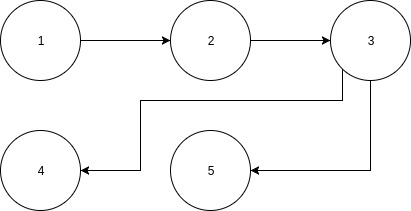
\includegraphics[width=5.5in,height=3.2in]{task.jpg}
\caption{Task Network}
\end{figure}
\newpage
\subsection{Timeline Chart}
\begin{figure}[!h]
\centering
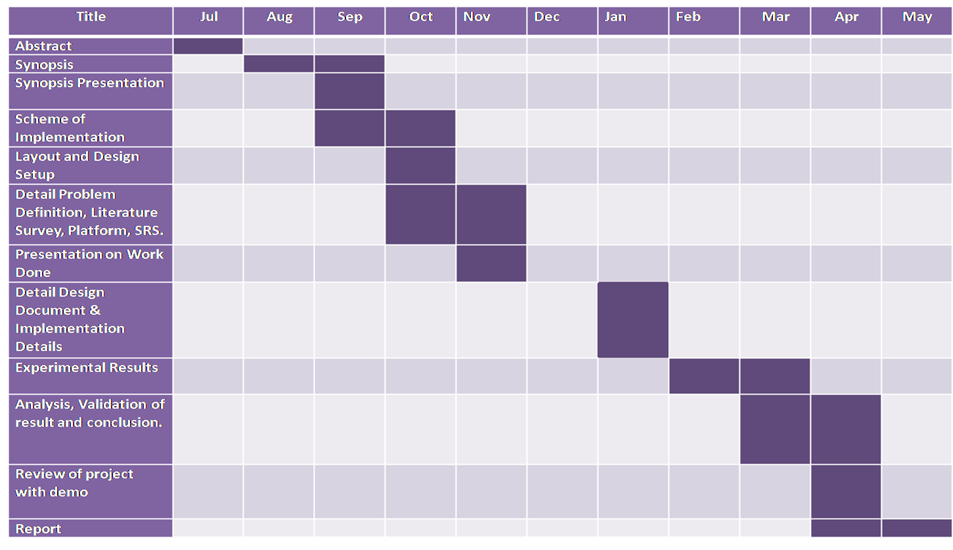
\includegraphics[width=5.5in,height=5.5in]{timeline.png}
\caption{Timeline Chart}
\end{figure}

\chapter{SOFTWARE REQUIREMENT SPECIFICATION}

\section{Introduction}
The aim of this document is to specify the software requirements for building a iterative behavioral model by analyzing candidate's tweets. 

\section{Purpose and Scope of the Document}
The purpose of the document is to enlist various software requirements to build the system. This document has functional and non-functional requirements for the software being developed.

\section{Overview of Responsibilities of Developer}
The responsibilities of a developer includes gathering of information about the classification libraries, that can be used to design and develop the system to categorize candidate's tweets. The developer’s responsibilities include: 
\begin{itemize}
\item Planning for dissertation (Scheduling) 
\item Designing of system (High Level Design Document)
\item Coding of system (Implementation)
\item Testing of system (Test Cases)
\end{itemize}

\section{Product Overview}
System builds a iterative behavioral model by fetching candidate's tweets and classifies them into one of the emotional categories and polarity categories. Different functionality of the system are : 

\begin{itemize}
\item Candidate Registration - It shows a registration page that candidate uses to registers for one of the organizations.
\item Candidate Data Downloading - It allows a Product Admin to download candidate's tweets from Twitter.
\item Candidate Profiling - Profiles are formed for specific candidate after analyzing tweets in the form of column graph. It shows percentage of emotional and polarity categories scores. Scores are shown year-wise, month-wise and day-wise.
\item Candidate Comparison - It allows Product Admin to compare two candidates with respect to their emotional and polarity scores achieved. Comparison graphs of candidates are shown year-wise, month-wise and day-wise.
\item Managing Candidate's Details and Data - It allows Product Admin to delete candidate's data or details or both.
\end{itemize}
\section{Hardware Resources Used}
4-Node Cluster with following configuration - 
\begin{itemize}
\item Intel(R) Core(TM) i5 CPU @ 2.90GHz or later, width : 64 bits 
\item Memory : 4 GB DDR3 or more 
\item Capacity : 1697MHz or more 
\item Cores : 4 or more 
\item PCI Express Gigabit Ethernet Controller, Size: 100Mbit/s, Capacity: 1Gbit/s, Width: 64 bits 
\item Hard Disk : 500 GB (EXT4 Primary/Logical Partition)
\end{itemize}


\section{Software Resources Used}
\begin{itemize}
\item OpenCV 3.0.0 or later
\item Python 2.7.6 or later
\item Ubuntu 14.04 or later
\item 
\item 

\end{itemize}

\section{Functionality}
\begin{itemize}
\item Fetch candidate's tweets from Twitter using Twitter API.
\item Show behavioral profile of candidates.
\begin{itemize}
\item Show percentage of emotional and polarity categories for specific candidate year-wise, month-wise and day-wise.
\item Show profile deviation of specific candidate.
\item Show positive, negative and offensive polarity score for specific candidates.
\end{itemize}
\item Show percentage of relevance to particular user defined requirements.
\item Compare two candidates for set of emotional and polarity categories.
\end{itemize} 

\section{Input}
\begin{itemize}
\item Dataset that consists of Twitter's tweets.
\item User specific requirements for finding relevance in candidate's profile.
\item Candidate's emotional and polarity categories score for comparison and profile generation.
\end{itemize}


\section{Output}
Candidate's behavioral profile that shows:
\begin{itemize}
\item Percentage of emotion and polarity categories
\item Relevance to particular user defined requirements.
\item Percentage of profile deviation.
\item Candidate's comparison graph.
\end{itemize}

\section{Major Constraints}

\begin{itemize}
\item To store candidate's data as an input in CSV format.
\item To store candidate's CSV file in Alluxio.
\item To form Spark Standalone Cluster. 
\item To execute Spark Classifier job in configured environment.
\item To train the model for emotional and polarity categories and store it in Alluxio.
\end{itemize}

\section{Applications}
\begin{itemize}
\item External candidates behavioral assessments visiting for recruitment drive or invited by
managers, organized by multiple organizations.
\item Internal candidates profile evaluation of multiple organizations.
\item HR Analytics.
\end{itemize}

\section{Usage Scenario}
A use case represents a particular functionality of a system. Hence, use case diagram is used to describe the relationships among the functionalities and their internal/external actors. This section provides various usage scenarios for the system to be developed.

\subsection{User Profiles}
Actors of the system are Candidate, Product Administrator, Storage System, Database System and Web Interface.
\begin{itemize}
    \item \textbf{Candidate} : Actor registers for a specific organization giving twitter URL and other details to Database using Web Interface.
    \item \textbf{Product Administrator} : Actor manages registers candidates, downloads tweets of a candidate, manages several behavioral assessment tests, profiles and compares candidates.
    \item \textbf{Storage System} : Actor stores tweets of candidates downloaded by Product Administrator.
    \item \textbf{Database System} : Actor stores emotional, polarity scores and other details of candidates.
    \item \textbf{Web Interface} : Actor displays candidate's emotional and polarity graphs according to year, month and day. It also allows Product Admin to download candidate's data and manage behavioral assessment tests.  
\end{itemize}
\newpage
\subsection{Use Cases}
Table 7.1 gives Use Cases for system to be developed.
\renewcommand{\arraystretch}{1.0}
\begin{table}[h]
\centering
\caption{Use Cases}
\label{my-label}
\begin{tabular}{|l|l|l|l|l|}
\hline
\textbf{Sr. No.} & \textbf{Use Case}                                                 & \textbf{Descriptions}                                                                                                                                                                                                    & \textbf{Actors}                                                                                                          & \textbf{Assumptions}                                                                                                    \\ \hline
1                & \begin{tabular}[c]{@{}l@{}}Candidate \\ Registration\end{tabular} & \begin{tabular}[c]{@{}l@{}}Candidate has to \\ registers for a \\ specific organization \\ giving necessary\\ details and saved \\ to Database.\end{tabular}                                                             & \begin{tabular}[c]{@{}l@{}}Candidate,\\ Database\\ System\end{tabular}                                                   & \begin{tabular}[c]{@{}l@{}}Provided\\ details \\ are correct\end{tabular}                                               \\ \hline
2                & \begin{tabular}[c]{@{}l@{}}Candidate Data\\ Download\end{tabular} & \begin{tabular}[c]{@{}l@{}}Product Admin \\ fetches candidate's\\  details from\\  database, Extract \\ screen name\\ from Twitter URL, \\ downloads candidate's \\ data and store it \\ in storage system.\end{tabular} & \begin{tabular}[c]{@{}l@{}}Candidate,\\ Database System, \\ Storage System,\\ Product\\ Admin\end{tabular}               & \begin{tabular}[c]{@{}l@{}}Data\\ is \\ downloaded\\  properly.\end{tabular}                                            \\ \hline
3                & \begin{tabular}[c]{@{}l@{}}Candidate \\ Comparison\end{tabular}   & \begin{tabular}[c]{@{}l@{}}Product Admin \\ chooses\\ two candidates\\ for comparison\\  based \\ on emotional and\\ polarity values.\end{tabular}                                                                       & \begin{tabular}[c]{@{}l@{}}Candidate,\\ Database System, \\ Product Admin, \\ Web Interface\end{tabular}                 & \begin{tabular}[c]{@{}l@{}}Comparison\\ between \\ two candidates \\ are \\ shown in the \\ form of graph.\end{tabular} \\ \hline
4                & \begin{tabular}[c]{@{}l@{}}Candidate \\ Profiling\end{tabular}    & \begin{tabular}[c]{@{}l@{}}Candidate are \\ profiled\\ based on set\\ of rules defined\\ by Product Admin.\end{tabular}                                                                                                  & \begin{tabular}[c]{@{}l@{}}Candidate,\\ Database System, \\ Product Admin, \\ Web Interface\end{tabular}                 & \begin{tabular}[c]{@{}l@{}}Profile\\ results are \\ displayed\\  in the form of \\ column graph.\end{tabular}           \\ \hline
5                & System                                                            & \begin{tabular}[c]{@{}l@{}}Overall \\ system\\ description\end{tabular}                                                                                                                                                  & \begin{tabular}[c]{@{}l@{}}Candidate,\\ Product Admin,\\ Database System,\\ Web Interface,\\ Storage System\end{tabular} & \begin{tabular}[c]{@{}l@{}}System\\ is\\ functional\end{tabular}                                                        \\ \hline
\end{tabular}
\end{table}
\newpage
\subsection{Use Case Views}
\subsubsection{Candidate Registration}
\begin{figure}[h!]
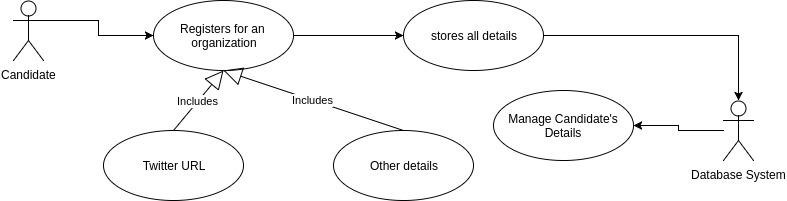
\includegraphics[width=5.2in,height=1.5in]{UseCase1.jpg}
\caption{Use Case : Candidate Registration}
\end{figure}
\subsubsection{Candidate Data Download}
\begin{figure}[h!]
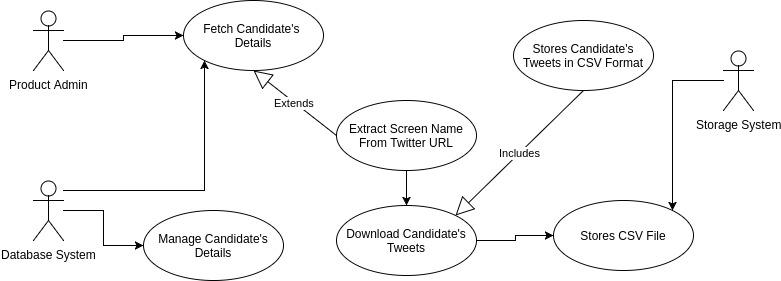
\includegraphics[width=5.2in,height=2.0in]{UseCase2.jpg}
\caption{Use Case : Candidate Data Download}
\end{figure}
\newpage
\subsubsection{Candidate Comparison}
\begin{figure}[h!]
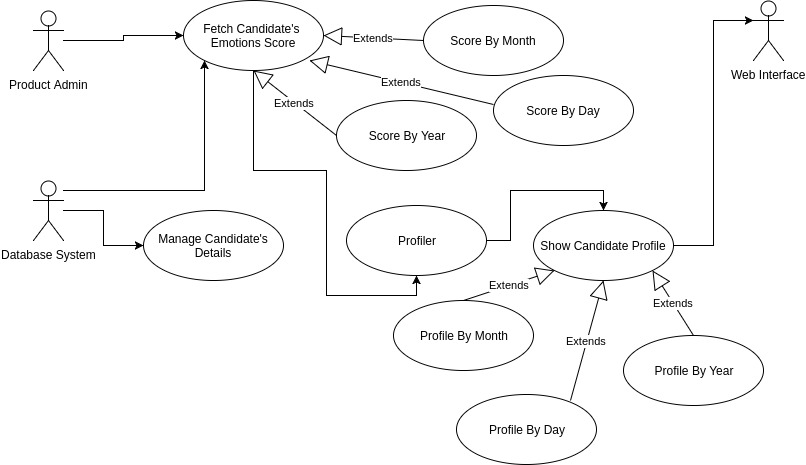
\includegraphics[width=5.2in,height=3.5in]{UseCase3.jpg}
\caption{Use Case : Candidate Comparison}
\end{figure}
\subsubsection{Candidate Profiling}
\begin{figure}[h!]
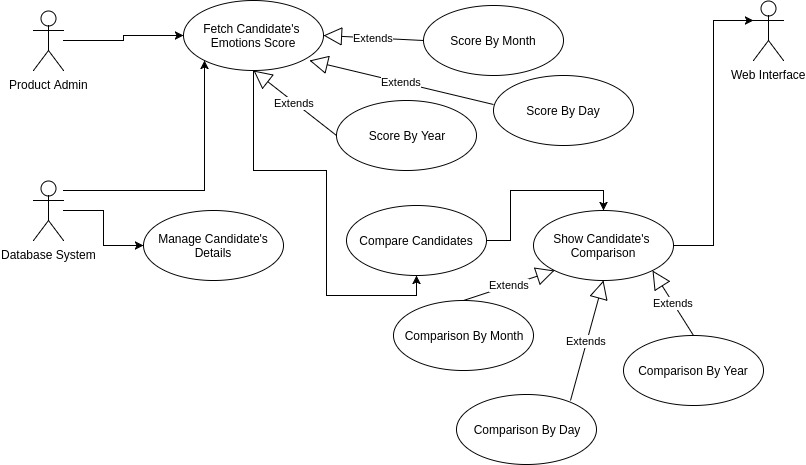
\includegraphics[width=5.2in,height=3.5in]{UseCase4.jpg}
\caption{Use Case : Candidate Profiling}
\end{figure}
\newpage
\subsubsection{System Use Case}
\begin{figure}[h!]
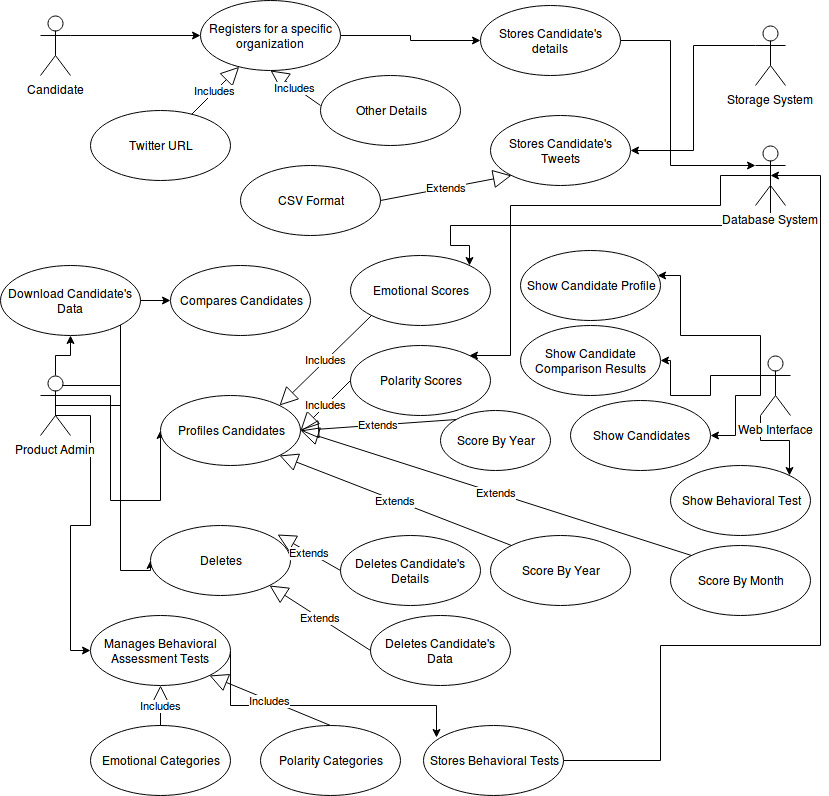
\includegraphics[width=5.2in,height=4.4in]{SystemUseCase.jpg}
\caption{Use Case : Overall System}
\end{figure}
\newpage
\section{Behavioral Model and Description}
This section contains details about events and associated behaviour of the system which is shown using diagram below.

\subsection{Activity Diagram}
Activity diagram is a flow chart to represent the flow form one activity to another activity. The activity can be described as an operation of the system. The control flow is drawn from one operation to another. This flow can be sequential, branched or concurrent. The purpose of activity diagrams is to capture the dynamic behaviour of the system.\\\\
\textbf{Description} : As shown in figure 7.6, Product Administrator downloads candidate's tweets from Twitter for analysis. Tweets are stored in a CSV format in Alluxio data storage. For analysis to take place, candidate's download status is check. If it is true, load candidate's CSV file and proceed with analysis else download candidate's tweets. For document classification, initially model existence is checked. If it exists, then load model for document classification else proceed with training phase. The training phase consists of document preprocessing, feature extraction and saving model in Alluxio. Classifier uses this trained model for document classification. Candidates are profiled and compared based on their document classified into emotional and polarity categories.
\begin{figure}[h!]
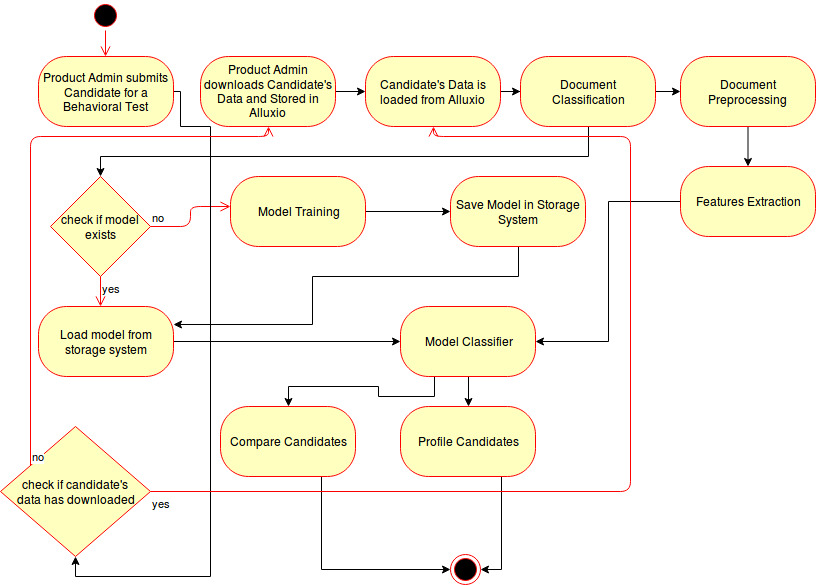
\includegraphics[width=5.0in,height=4.0in]{Activity.jpg}
\caption{Activity Diagram}
\end{figure}
\newpage
\section{Functional Model and Description}
This section describes data flow diagrams (DFD) of the proposed system. There are three types of DFDs explained in the section. These diagrams explain the system in brief.

\subsection{Data Flow Diagram}
\subsubsection{Level 0 Data Flow Diagram}
In the level 0 DFD as shown in figure 7.7, Candidates registers into Behavioral Assessment System. System performs analysis and generates reports for a registered candidate. They are displayed to Product Admin.\\
\begin{figure}[h!]
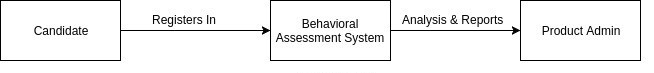
\includegraphics[width=4.5in]{DFD-0.jpg}
\caption{Level 0 DFD}
\end{figure}

\subsubsection{Level 1 Data Flow Diagram}
In the level 1 DFD as shown in figure 7.8, Candidate's tweets are fetched from Twitter by Product Admin using Web Interface. Tweets are stored in Alluxio for storage. They are retrieved by Web Application modules for analysis and report generation.\\
\begin{figure}[h!]
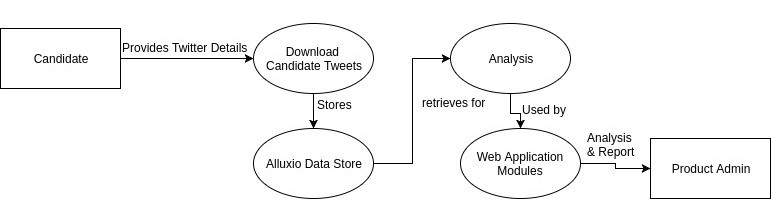
\includegraphics[width=4.5in]{DFD-1.jpg}
\caption{Level 1 DFD}
\end{figure}

\subsubsection{Level 2 Data Flow Diagram}
In the level 2 DFD as shown in figure 7.9, Candidate's tweets are retrieved from Alluxio Data Storage and preprocessed. Features are extracted for Classification. It classifies tweets of a candidate to emotional and polarity categories. Candidate are profiled and compared based on these categories. Profile and comparison results are displayed to Product Admin using Web Interface.\\
\begin{figure}[h!]
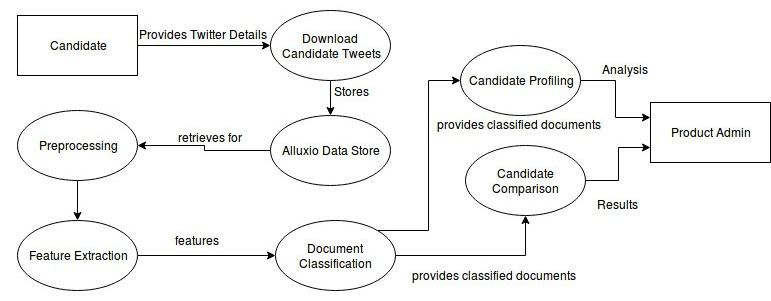
\includegraphics[width=4.5in]{DFD-2.jpg}
\caption{Level 2 DFD}
\end{figure}
\\
\section{Non-Functional Requirements}
\subsection{Availability}
Internet connection is needed as Bootstrap, J Query libraries are fetched from their respective Content Delivery Network. It is also required to fetch candidate's tweets from Twitter.

\subsection{Scalability}
The system should be scalable to connect more number of Spark nodes if candidate's data is increased. Apache Spark is configured to connect more nodes if need arises.

\subsection{Performance}
The system must be interactive and delays involved must be less. There should be no immediate delays for every action and response of the system. In web application, flash success and error messages generate delay of 1 second. Execution request sent from web application to spark application should involve minimal delay. Execution time of Spark application depends upon processing of candidate's tweets stored in CSV format. It should take less time as multiple nodes are connected for processing.

\subsection{Security}
A product administrator should be able to securely login to web application and submit candidate's tweets for analysis. Hadoop, Alluxio and Spark components must interact with each other in a secure manner.

\subsection{Usability}
The system should be easy to handle and process requests efficiently. System's functions are designed to use with ease and provide results. Candidate's analysis reports are presented in the form of graph and easy to comprehend.

\subsection{Reliability}
The system should efficiently analyze candidate's tweets entirely and stores all the classified documents to database. It should be reliable to perform web application requests, receive responses and perform actions based on responses without fail. Kerberos Authentication is implemented for mutual authentication between processing components of computational framework and storage systems to secure candidate's information. 

\subsection{Maintainability and Changeability}
The system is made up of different independent modules that can be modified to correct faults, improve performance or other attributes, or adapt to a changed environment. System can be improved for new features and will be able to include new requirements.

\chapter{DETAILED DESIGN DOCUMENT}

\section{Introduction}
This document specifies the design that is used to fetch candidate tweets in CSV format, classifies individual tweets into emotion and polarity categories, profiles candidates based on predefined rules and predict future behavior of candidate.

\section{Behavioral Modeling}
Candidate's tweets are classified into emotional and polarity categories. Over the course of candidate's social media presence, profile deviates that forms a iterative behavioral model.
\begin{itemize}
    \item \textbf{Emotional Categories}
    \begin{itemize}
        \item Anger
        \item Disgust
        \item Joy
        \item Love
        \item Fear
        \item Sadness
        \item Surprise
    \end{itemize}
    \item \textbf{Polarity Categories}
    \begin{itemize}
    \item Positive
    \item Negative
    \item Offensive
    \end{itemize}
\end{itemize}
Candidate's tweets are collected and classified based on these categories. They are profiled and compared based on emotional and polarity categories.
\newpage
\section{Architectural Design}
\begin{figure}[!h]
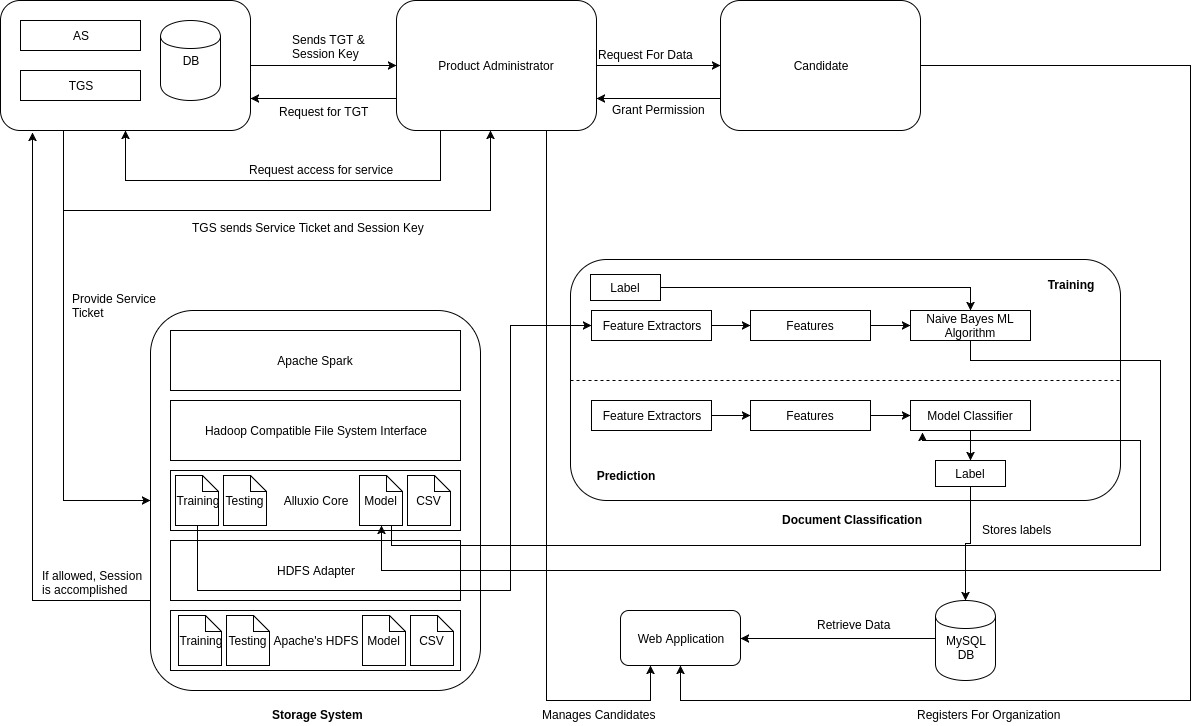
\includegraphics[width=5.7in,height=4.0in]{Architecture.jpg}
\caption{Proposed System Architecture}
\end{figure}
Figure 7.1 shows architectural design of proposed system. Following are important components in the system :
\begin{itemize}
\item Storage System : Alluxio, memory centric storage system is used as main storage system which stores in-memory data. Apache's HDFS is used as an underFS storage system. Candidate's CSV files, trained models, testing and training dataset is stored in Alluxio.
\item Computation Framework : Apache's Spark is used for computations. Document classifier is built in Spark. It access candidate's CSV, trained model files from Alluxio. Spark's Mlib is used for training Naive Bayes model which is stored in Alluxio after training.
\item Document Classifier : First, Naive Bayes model is trained by training dataset of emotional and polarity categories and saved in Alluxio. After training, prediction stage occurs. It access candidate's CSV file from Alluxio and classifies document on each candidate's tweet. Predicted labels on each tweet is stored in MySQL database with year, month and day.
\item Candidate registers for specific organization using web application, providing twitter details. Product Administrator access web application to download candidate's tweets from Twitter, manages candidates, profiles and compares candidates. 
\item Kerberos is  used for mutual authentication between storage system components and document classifier. It consists of Authentication Server, Database and Ticket Granting Service. Product Administrator requests Key Distribution Center for a valid ticket before submitting Spark job. If no valid ticket found, operation is not permitted. With only valid ticket, candidate's tweets are analyzed.  
\end{itemize}
\section{Class Design}
It is a static diagram that represents the static view of an application. It is not only used for visualizing, describing, and documenting different aspects of a system but also for constructing executable code of the software application. It describes the attributes and operations of a class and also the constraints imposed on the system.\\\\
\textbf{Description} : In figure 8.2, modules and their relationships are shown. Document classifier used for classifying candidate's tweets takes user identifier of candidate and candidate's CSV location in Alluxio as an input. Product Administrator fetches candidate's tweets from Twitter in a CSV format and store the file in Alluxio. Candidate's CSV file location is saved into database for further processing. After document classification, candidates can be profiled and compared based on their emotional and polarity categories. For both modules, results are displayed by year, month and day.
\begin{figure}[h!]
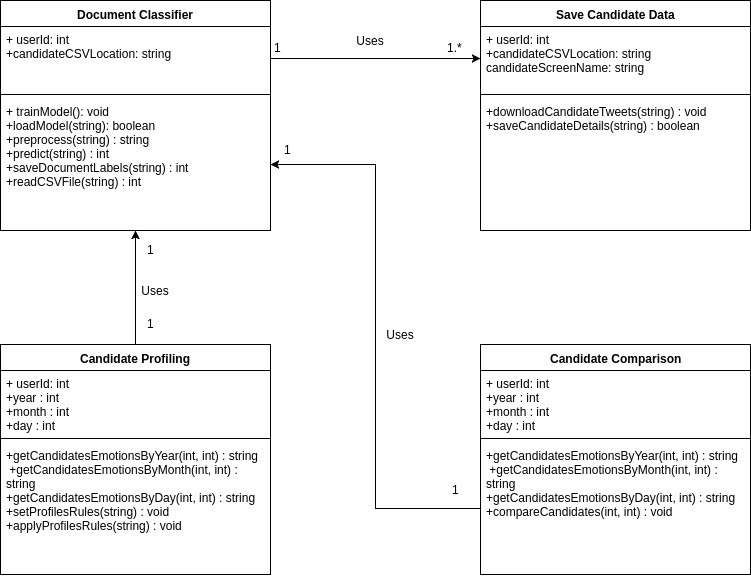
\includegraphics[width=4.5in,height=4.0in]{Class.jpg}
\caption{Class Diagram}
\end{figure}
\newpage
\section{Component Design}
It is used to model the physical aspects of a system. It is also used to visualize the organization and relationships among components in a system. It does not describe the functionality of the system but it describes the components used to make those functionalities.\\\\
\textbf{Description} : Figure 8.3 describes primary components of the system. A web application provides candidate's tweets to be fetched and candidates are profiled and compared functionality to Product Administrator. Product Admins are authenticated first before using any of the functionality. To download tweets of a specific candidate, he/she must register for that organization. Tweets are stored in Alluxio data storage in CSV format. Data storage is accessed by Spark application for fetching candidate's tweets for preprocessing and document classification. 
\begin{figure}[h!]
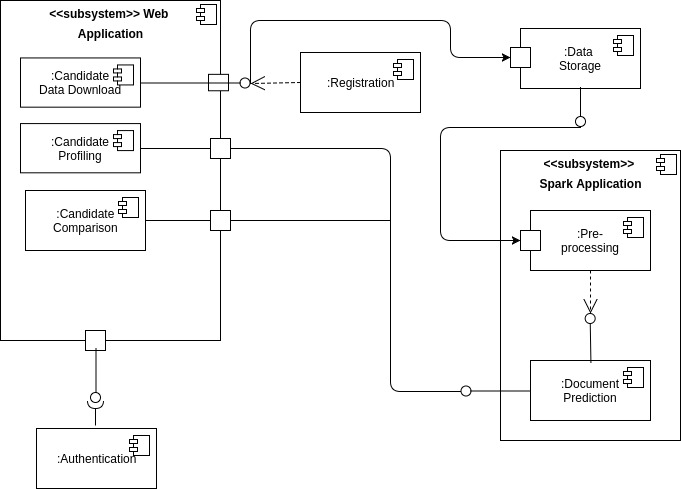
\includegraphics[width=5.2in,height=4.2in]{component.jpg}
\caption{Component Diagram}
\end{figure}
\section{Deployment Design}
 It is used visualize the topology of the physical components of a system, where the software components are deployed. It describes the static deployment view of a system, consisting of nodes and their relationships.\\\\
 \textbf{Description} : In figure 8.4, Web application designed in Laravel PHP runs on Apache Tomcat Server. Process component of Symphony is used to run spark application. 4-Node cluster is formed for spark application execution. It requires data from Alluxio data storage system. Alluxio is specifically compiled for Spark for data access. Web application retrieves candidate's emotional and polarity scores from database.
\begin{figure}[h!]
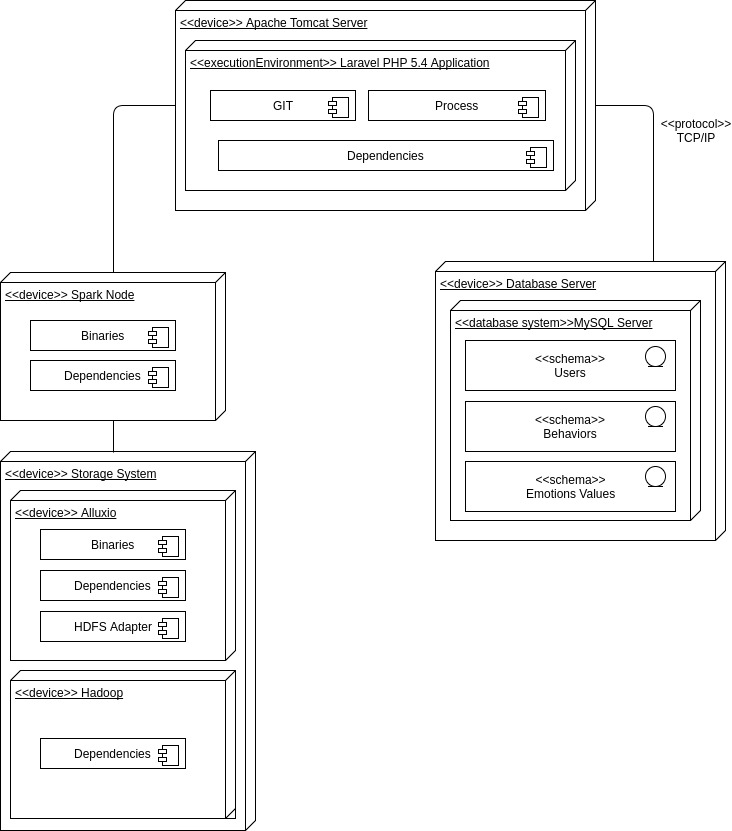
\includegraphics[width=5.2in,height=4.2in]{Deployment.jpg}
\caption{Deployment Diagram}
\end{figure}

\chapter{IMPLEMENTATION DETAILS}
\section{Introduction}
This section describes implementation of the system, required libraries and dependencies needed for components of the system and use of implementation strategy.
\section{Algorithm}
\subsection{Document Classification}

\textbf{Input} : Candidate's CSV file and Unique Identifier. \\
\textbf{Output} : Candidate's tweets classified into emotional and polarity categories. \\\\
Initialize numFeatures to 10000 \\
Initialize emotionalTrainingDataPath to /emotion-training \\  
Initialize polarityTrainingDataPath to /polarity-training \\
Initialize emotionModel to /emotion-model \\
Initialize polarityModel to /polarity-model \\
Input candidateCSVLocation \\
Input candidateUserId \\\\
If  emotionModel exists
    \par load emotionModel\\
Else
    \par load Category Data from emotionalTrainingDataPath
	\par transform Category Data using Hashing Transform for numFeatures
	\par attach label to Category Data
	\par save emotionModel to /emotion-model
	\par load emotionModel from /emotion-model\\
If  polarityModel exists
	\par load polarityModel \\
Else
	\par load Category Data from polarityTrainingDataPath
	\par transform Category Data using Hashing Transform for numFeatures
	\par attach label to Category Data
	\par save polarityModel to /polarity-model
	\par load polarityModel from /polarity-model\\
Read CSV file from candidateCSVLocation\\
While CSV file contains some rows
	\par Read Columns from CSV file
	\par Column 0 contains 'Date'
	\par Column 1 contains 'Actual Tweet'
	\par Split Column 0 into year, month and day
	\par Transform Column 1 using Hashing Transform for numFeatures
	\par Classify Column 1 with respect to emotionModel and get emotionLabel
	\par Save emotionLabel into database with year, month and day
	\par Classify Column 1 with respect to polarityModel and get polarityLabel
	\par Save polarityLabel into database with year, month and day

\subsection{Candidate Profiling}
\textbf{Input} : Candidate's User Identifier.\\
\textbf{Output} : Candidate Profiles\\\\
Input Candidate's User Identifier.\\
Retrieve years from Database based on UserId\\
Retrieve months from Database based on UserId\\
Retrieve days from Database based on UserId\\\\
\textbf{Calculate Percentage of Categories for all years}\\
Retrieve emotionsValues from Database based on UserId for all years\\
Retrieve polarityValues from Database based on UserId for all years\\\\
While candidate has emotion category and value in a year
	\par Calculate Total number of documents in a year
	\par Calculate Total number of document for a specific category
	\par Calculate Percentage for a specific category\\
While candidate has polarity category and value in a year
	\par Calculate Total number of documents in a year
	\par Calculate Total number of document for a specific category for a year
	\par Calculate Percentage for a specific category for a year\\\\
\textbf{Calculate Percentage of Categories for all months}\\
Retrieve emotionsValues from Database based on UserId for all months group by years\\
Retrieve polarityValues from Database based on UserId for all months group by years\\\\
While candidate has emotion category and value in a month for specific year
	\par Calculate Total number of documents in a month
	\par Calculate Total number of document for a specific category
	\par Calculate Percentage for a specific category for a month\\
While candidate has polarity category and value in a month for specific year
	\par Calculate Total number of documents in a month
	\par Calculate Total number of document for a specific category for a year
	\par Calculate Percentage for a specific category for a month\\\\
\textbf{Calculate Percentage of Categories for all days}\\\\
Retrieve emotionsValues from Database based on UserId for all days in a month for a specific year\\
Retrieve polarityValues from Database based on UserId for all days in a month for a specific year\\\\
While candidate has emotion category and value for all days in a month for specific year
	\par Calculate Total number of documents in a day
	\par Calculate Total number of document for a specific category
	\par Calculate Percentage for a specific category for a day\\
While candidate has polarity category and value for all days in a month for specific year
	\par Calculate Total number of documents in a day
	\par Calculate Total number of document for a specific category
	\par Calculate Percentage for a specific category for a day
\section{Modules}
\subsection{Candidate's Tweets Fetched From Twitter}
\begin{itemize}
\item This modules retrieves candidate's tweets from Twitter. Input to module is candidate's screen name. 
\item Every user in twitter has unique screen name which can be used to retrieve his/her tweets using Twitter APIs and OAuth. 
\item OAuth 2 is an authorization framework that enables application to obtain limited access to user accounts on an HTTP service such as Facebook and Twitter. 
\item A Twitter application is created, python module connects to Twitter application using consumer secret key and consumer key. Twitter application also generates access key and access secret key which decides validity of tweets access. Tweets are fetch and store it in CSV format. 
\item The CSV file of every candidate is pushed to Alluxio storage system. Python's Tweepy library is used for implementation of this module. 
\item A Product Administrator uses candidate data downloading functionality to trigger this module giving candidate's screen name as an input.
\end{itemize}
\subsection{Document Classification}
\begin{itemize}
\item This module takes candidate's CSV location in Alluxio and unique identifier as an input. 
\item This module is written in Scala and executes as an spark job on multi-node spark cluster. This means, spark job uses resources of multiple connected nodes for faster processing. 
\item Alluxio is memory centric distributed storage system that provides candidate's CSV file to spark job. Spark's Machine Learning library is used for  implementation of Naive Bayes Classifier. 
\item Initially, model is trained by training dataset that consists of emotional categories of 21429 records and polarity categories of 8797 records. Both models are saved to and loaded from Alluxio. 
\item Every candidate's tweet is classified into one of the emotional and polarity categories. A database insertion operation push classified documents along with user identifier to MySQL.
\end{itemize}

\subsection{Web Application}
Web application is designed and built in Laravel PHP 5.4. High charts is used for showing candidate results in the form of column graphs. There are different modules in web application - 
\begin{itemize}
\item Candidate Profiling : Module shows each candidate's emotional and polarity categories percentage year-wise, month-wise and day-wise.
\item Candidate Comparison : Two candidates are compared by emotional and polarity categories percentage. Results are shown year-wise, month-wise and day-wise.
\item Candidate Data Downloading Functionality : It enables product administrator to download tweets of a certain candidate. It uses Process component of Symphony to execute python script that fetches tweets from Twitter.
\item Storage Analyzer : It shows storage space used by candidate's CSV files, training and testing dataset and saved trained models in Alluxio. Alluxio's local file system commands are used to retrieve space occupied. 
Registration – It allows a candidate to register himself/herself to a certain organization. 
\item Assessment creation and deletion : Assessments are created, deleted and updated by product administrator. 
\end{itemize}

\section{Dataset}
\hspace{1.1cm}Dataset comprises of tweets from Twitter. It has to be collected for every candidate that needs to be assessed for behavioural assessment. There is significant latency and load on server in fetching such information of candidate using Twitter API.
\par After the dataset is collected, it needs to be stored in underFS storage layer. Movement of huge dataset to storage layer requires additional I/O writes and communication overhead. But, by using proposed system, writes operation to storage layer is significantly lesser.
\par For document classification, a training and testing dataset is required. Training records for emotional and polarity categories are mentioned in Table 9.1 and 9.2.

\renewcommand{\arraystretch}{1.5}
\begin{table}[h!]
\centering
\caption{Emotional Training Dataset}
\label{my-label}
\begin{tabular}{|l|l|}
\hline
\textbf{Emotion Category} & \textbf{Training Records} \\ \hline
Anger                     & 1572                      \\ \hline
Joy                       & 8276                      \\ \hline
Disgust                   & 761                       \\ \hline
Love                      & 216                       \\ \hline
Sadness                   & 3853                      \\ \hline
Surprise                  & 3912                      \\ \hline
Fear                      & 2839                      \\ \hline
\textbf{Total}            & \textbf{21429}            \\ \hline
\end{tabular}
\end{table}

\begin{table}[h!]
\centering
\caption{Polarity Training Dataset}
\label{my-label}
\begin{tabular}{|l|l|}
\hline
\textbf{Polarity} & \textbf{Training Records} \\ \hline
Positive          & 2007                      \\ \hline
Negative          & 4783                      \\ \hline
Disgust           & 2007                      \\ \hline
\textbf{Total}    & \textbf{8797}             \\ \hline
\end{tabular}
\end{table}


\section{Snapshots}

\chapter{TEST SPECIFICATION}

\section{Introduction}
This document explains the test plan and testing strategy for modules in a system. Following modules needs to be tested - 
\begin{itemize}
\item Fetching candidate's tweets from Twitter and store it in CSV format.
\item Classification of candidates in emotional and polarity categories.
\item Web application that sends requests, collect responses and act based on responses.
\end{itemize}

\subsection{Goals and Objectives}
\begin{itemize}
\item To validate candidate's tweets in a CSV after fetching it from Twitter.
\item To check accuracy of different document classifiers.
\item To validate predicted document labels of candidate's tweets.
\item To validate candidate's profiles and comparison results.
\item To validate execution distribution among multiple connected nodes.
\end{itemize}

\subsection{Statement of Scope}
Testing will be done on individual modules of a system. Testing will be carried out for several different candidates. Finally, system as a whole is tested for correctness of results. 

\subsection{Major Constraints}
Testing is done manually. For testing the accuracy of document classifiers, testing dataset is formed and used. Total number of multiple connected nodes is limited to four nodes.

\section{Test Plan}
\subsection{Modules to be Tested}
\begin{itemize}
\item Candidate's tweets fetched from Twitter module.
\item Candidate's tweets classification module.
\item Web Application.
\end{itemize}

\subsection{Testing Strategy}
\subsubsection{Unit Testing}
Unit testing has been done for all the individual modules. While doing unit testing different parameter has been considered and according to input to the system different output is recorded. After recording output of unit testing different solution are applied to pass the test. This is carried out as white box testing.
\begin{itemize}
\item To test candidate's tweets are fetched and stored in a CSV format.
\item To test classification module's effectiveness and prediction of document labels.
\item To test different classifier's accuracy.
\item To test candidate profiles and comparison's results. Result must be shown in the form of graph.
\item To test candidate's documents analysis occurs distributively, using resources of multiple connected nodes. 
\end{itemize}

\subsubsection{Integration Testing}
Once unit testing is complete for individual modules, all the modules are integrated together and tested for functional correctness. While doing integration testing, developer has kept in mind few constraints which need to be achieved in order to get desired results.
\begin{itemize}
\item Web application requests needs to be accepted by classification module and response back with predicted document labels for candidate's tweets.
\item Web application uses candidate's data download functionality to fetch candidate's tweets from Twitter and store it in Alluxio.
\item Web Application retrieves candidate's analysis results and forms a column b ar graph.
\item Candidates are compared for seven emotional categories and results are shown as a graph.
\end{itemize}

\subsubsection{Validation Testing}
Validation testing is carried out to test the entire work flow and input validation. This is carried out as a black box testing. In this project validation testing has been conducted on different modules.
\begin{itemize}
\item To validate candidate's tweets in a CSV after fetching it from Twitter.
\item To validate predicted document labels of candidate's tweets.
\item To validate candidate's profiles and comparison results.
\item To validate execution distribution among multiple connected nodes.
\end{itemize}

\subsubsection{System Testing}
\begin{itemize}
\item To test if all GUI elements are shown properly in a web interface.
\item To test if spark application is executed atomically using web interface.
\item To test if spark application is able to access data stored in Alluxio.
\item To test if Kerberos is integrated into Spark and Alluxio.
\end{itemize}

\subsubsection{GUI Testing}
Front End of the system is designed as web application, runs on local server. Data visualization is provided by High charts. \\
Following modules needs to be tested in a web application - 
\begin{itemize}
\item Candidate's data downloading functionality
\item Assessment creation and deletion
\item Storage Analyzer
\item Candidate's profiles
\item Candidates comparison 
\end{itemize}

\subsubsection{High Order Testing}
It includes carrying out performance testing by checking complete running time of document classification on multinode spark cluster.

\subsection{Test Procedure}
\subsubsection{Unit Testing}
\begin{table}[h!]
\centering
\caption{Unit Test Cases}
\begin{tabular}{|l|l|l|l|l|}
\hline
\textbf{Sr. No.} & \textbf{\begin{tabular}[c]{@{}l@{}}Test Case \\ Name\end{tabular}}               & \textbf{\begin{tabular}[c]{@{}l@{}}Test Case\\ Objective\end{tabular}}                                                                       & \textbf{\begin{tabular}[c]{@{}l@{}}Test Case\\ Input\end{tabular}}                        & \textbf{\begin{tabular}[c]{@{}l@{}}Test Case\\ Result\end{tabular}} \\ \hline
1                & Log In                                                                           & \begin{tabular}[c]{@{}l@{}}Product Admin should\\ be able to log in for\\ correct organization\\ only.\end{tabular}                          & \begin{tabular}[c]{@{}l@{}}Username \&\\ Password\end{tabular}                            & Pass                                                                \\ \hline
2                & \begin{tabular}[c]{@{}l@{}}View\\ Candidates\end{tabular}                        & \begin{tabular}[c]{@{}l@{}}Product Admin should \\ be able to view all\\ candidates registered\\ for organization.\end{tabular}              & \begin{tabular}[c]{@{}l@{}}Candidate's\\ Details\end{tabular}                             & Pass                                                                \\ \hline
3                & \begin{tabular}[c]{@{}l@{}}Create \\ Behavioral\\ Assessment\\ Test\end{tabular} & \begin{tabular}[c]{@{}l@{}}Product Admin should\\ be able to create\\ customized behavioral\\ test.\end{tabular}                             & \begin{tabular}[c]{@{}l@{}}Emotional and\\ polarity\\ categories's \\ values\end{tabular} & Pass                                                                \\ \hline
4                & \begin{tabular}[c]{@{}l@{}}Candidate\\ Registration\end{tabular}                 & \begin{tabular}[c]{@{}l@{}}Candidate should be\\ able to register for \\ specific organization.\end{tabular}                                 & \begin{tabular}[c]{@{}l@{}}Candidate's\\ Details\end{tabular}                             & Pass                                                                \\ \hline
5                & \begin{tabular}[c]{@{}l@{}}Manage \\ Candidate\\ Data\end{tabular}               & \begin{tabular}[c]{@{}l@{}}Product Admin should\\ be able to delete \\ candidate's records \\ and tweets stored in\\ CSV format\end{tabular} & \begin{tabular}[c]{@{}l@{}}Candidate's\\ User Identifier\end{tabular}                     & Pass                                                                \\ \hline
\end{tabular}
\end{table}
\subsubsection{Integration Testing}
\begin{table}[h!]
\centering
\caption{Integration Test Cases}
\begin{tabular}{|l|l|l|l|l|}
\hline
\textbf{Sr. No.} & \textbf{\begin{tabular}[c]{@{}l@{}}Test Case \\ Name\end{tabular}} & \textbf{\begin{tabular}[c]{@{}l@{}}Test Case\\ Objective\end{tabular}}                                                                                                    & \textbf{\begin{tabular}[c]{@{}l@{}}Test Case\\ Input\end{tabular}}                    & \textbf{\begin{tabular}[c]{@{}l@{}}Test Case\\ Result\end{tabular}} \\ \hline
1                & \begin{tabular}[c]{@{}l@{}}Candidate\\ Profiling\end{tabular}      & \begin{tabular}[c]{@{}l@{}}Product Admin\\ submits candidate's\\ tweets for profiling.\\ Emotional and polarity\\ scores must be generated\\ after analysis.\end{tabular} & \begin{tabular}[c]{@{}l@{}}Candidate's \\ Unique\\ Identifier\end{tabular}               & Pass                                                                \\ \hline
2                & \begin{tabular}[c]{@{}l@{}}Candidate\\ Comparison\end{tabular}     & \begin{tabular}[c]{@{}l@{}}Product Admin selects two\\ candidates for comparison.\\ Comparison occurs based on\\ emotional and polarity scores.\end{tabular}              & \begin{tabular}[c]{@{}l@{}}Unique User\\ identifier \\ of both candidates.\end{tabular} & Pass                                                                \\ \hline
\end{tabular}
\end{table}
\newpage
\subsubsection{Validation Testing}
\begin{table}[h!]
\centering
\caption{Validation Test Cases}
\begin{tabular}{|l|l|l|l|l|}
\hline
\textbf{Sr. No.} & \textbf{\begin{tabular}[c]{@{}l@{}}Test Case \\ Name\end{tabular}}                                 & \textbf{\begin{tabular}[c]{@{}l@{}}Test Case\\ Objective\end{tabular}}                                                                                   & \textbf{\begin{tabular}[c]{@{}l@{}}Test Case\\ Input\end{tabular}}                                  & \textbf{\begin{tabular}[c]{@{}l@{}}Test Case\\ Result\end{tabular}} \\ \hline
1                & \begin{tabular}[c]{@{}l@{}}Candidate\\ Data\\ Validation\end{tabular}                              & \begin{tabular}[c]{@{}l@{}}Candidate's details\\ are first validated\\ against rules set.\end{tabular}                                                   & \begin{tabular}[c]{@{}l@{}}Candidate's\\ details.\end{tabular}                                      & Pass                                                                \\ \hline
2                & \begin{tabular}[c]{@{}l@{}}Candidates\\ listing for\\ Behavioral\\ Assessment\\ Tests\end{tabular} & \begin{tabular}[c]{@{}l@{}}Candidates whose\\ tweets are fetched \\ should only appear \\ in list for test.\end{tabular}                                 & \begin{tabular}[c]{@{}l@{}}Candidate's\\ Twitter Data\\ Download\\ Status\end{tabular}              & Pass                                                                \\ \hline
3                & \begin{tabular}[c]{@{}l@{}}Candidate\\ listing for\\ Profiling and\\ Comparison\end{tabular}       & \begin{tabular}[c]{@{}l@{}}Candidates whose\\ tweets have been \\ analyzed should only\\ appear in list for \\ profiling and \\ comparison.\end{tabular} & \begin{tabular}[c]{@{}l@{}}Candidate's\\ Behavioral\\ Assessment\\ Completion\\ Status\end{tabular} & Pass                                                                \\ \hline
\end{tabular}
\end{table}
\newpage
\subsubsection{System Testing}
\begin{table}[h!]
\centering
\caption{System Test Cases}
\label{my-label}
\begin{tabular}{|l|l|l|l|l|}
\hline
\textbf{Sr. No.} & \textbf{\begin{tabular}[c]{@{}l@{}}Test Case \\ Name\end{tabular}}           & \textbf{\begin{tabular}[c]{@{}l@{}}Test Case\\ Objective\end{tabular}}                                                                                                                      & \textbf{\begin{tabular}[c]{@{}l@{}}Test Case\\ Input\end{tabular}}             & \textbf{\begin{tabular}[c]{@{}l@{}}Test Case\\ Result\end{tabular}} \\ \hline
1                & \begin{tabular}[c]{@{}l@{}}GUI elements\\ displayed\\ properly.\end{tabular} & \begin{tabular}[c]{@{}l@{}}To show all GUI\\ elements in Web\\ Interface properly\end{tabular}                                                                                              & Views                                                                          & Pass                                                                \\ \hline
2                & \begin{tabular}[c]{@{}l@{}}Executing\\ Spark\\ Application\end{tabular}      & \begin{tabular}[c]{@{}l@{}}Web application\\ executes Spark\\ application for tweets\\ classification into\\ emotional and polarity\\ categories.\end{tabular}                              & \begin{tabular}[c]{@{}l@{}}Candidate's\\ Unique\\ User Identifier\end{tabular} & Pass                                                                \\ \hline
3                & \begin{tabular}[c]{@{}l@{}}Alluxio data\\ access\end{tabular}                & \begin{tabular}[c]{@{}l@{}}Spark application\\ accesses tweets stored\\ in CSV format\\ from Alluxio.\end{tabular}                                                                          & \begin{tabular}[c]{@{}l@{}}Candidate's\\ Unique User\\ Identifier\end{tabular} & Pass                                                                \\ \hline
4                & \begin{tabular}[c]{@{}l@{}}Kerberos\\ Authentication\end{tabular}            & \begin{tabular}[c]{@{}l@{}}Product Admin must be\\ authenticated first and \\ should have valid ticket, \\ before submitting\\ candidate's tweets for\\ analysis.\\ submitting\end{tabular} & \begin{tabular}[c]{@{}l@{}}Product Admin's\\ Keytab\end{tabular}               & Pass                                                                \\ \hline
\end{tabular}
\end{table}
\chapter{DATA TABLES AND DISCUSSIONS} 
\section{Kerberos Sub-System Analysis}
\hspace{1.1cm}A client may submit only one MR job or multiple jobs at a same time. The number of communication rounds and total number of protocol messages generated for different numbers of MR-Request-Component can be calculated. As number of jobs submission increases so does the communication overhead. There are three different use cases-
\begin{itemize}
\item One client can submit one job for submission.
\begin{itemize}
\item Total number of components requesting access to MR Resource for this case-
\begin{equation}
1(C) + n(Comp)
\end{equation}
\item Total number of communication rounds from Authentication Server to MR-Request-Component-
\begin{equation}
2(R) + 2n(R)
\end{equation}
\item Total number of communication rounds from MR-Request-Component to MR-Resource-Component are-
\begin{equation}
1(R) + n(R)
\end{equation}
\item Total number of messages sent are-
\begin{equation}
6 + 6n
\end{equation}
\end{itemize}
\item One client can submit multiple jobs for submission.
\begin{itemize}
\item Total number of components requesting access to MR Resource for this case-
\begin{equation}
1(C) + z \times n(Comp)
\end{equation}
\item Total number of communication rounds from Authentication Server to MR-Request-Component-
\begin{equation}
2(R) + z \times 2n(R)
\end{equation}
\item Total number of communication rounds from MR-Request-Component to MR-Resource-Component are-
\begin{equation}
1(R) + z \times n(R)
\end{equation}
\item Total number of messages sent are-
\begin{equation}
6 + 6n \times z
\end{equation}
\end{itemize}
\item Multiple client can submit multiple jobs for submission.
\begin{itemize}
\item Total number of components requesting access to MR Resource for this case-
\begin{equation}
y(C) + y \times z \times n(Comp)
\end{equation}
\item Total number of communication rounds from Authentication Server to MR-Request-Component-
\begin{equation}
y \times 2(R) + y \times z \times 2n(R)
\end{equation}
\item Total number of communication rounds from MR-Request-Component to MR-Resource-Component are-
\begin{equation}
1(R) + y \times z \times n(R)
\end{equation}
\item Total number of messages sent are-
\begin{equation}
6y + 6y \times n \times z
\end{equation}
\end{itemize}
\end{itemize}
One Client (C) has on Job(J) with n Components (Comp) per job. One Client has z jobs with n Components (Comp) per job. y Clients, each client has z jobs with n Component (Comp) per job. 
\par For a N number of MR components requests access to MR-Resource-Component per job,
number of communication rounds and messages for an authentication process can be calculated as,
\begin{itemize}
\item For communication round from Authentication Server to MR-Request-Component Communication
\begin{equation}
2N \times R (2N \times Request + 2N \times Response)
\end{equation}
\item For communication round from MR-Request-Component to MR-Resource-Component
\begin{equation}
N \times R (N \times Request + N \times Response)
\end{equation}
\end{itemize}

\section{Alluxio Storage System Performance Analysis}
\hspace{1.1cm}For writes throughput, Alluxio outperforms MemHDFS by 110x and for reads throughput, 2x greater than MemHDFS. It's read throughput is higher than write throughput. This happens due to machine configured with optimized memory hardware, leaving more bandwidth for reads.
\par It also improves the end-to-end latency of a realistic work flow by 4x. Introducing check-pointing algorithm guarantees recovery cost and resource allocation strategies for re-computation under resource schedulers.
\par Alluxio architecture consists of two layers- lineage and persistence. The
lineage layer provides high throughput I/O and tracks the sequence of jobs that have created a particular data output. The persistence layer persists data onto storage without the lineage concept.


\chapter{CONCLUSION}
We proposed a hand gesture based human computer
interaction system that provides a  natural  way to interact with computer.The hand is first segmented  by using skin color information and then tracked using 'Camshift' tracker with Kalman filter, then fingertips are located on the contour of the segmented hand and single gestures drawn from fingertips are recognized. For  pointing, click, right click, zoom, drag and window closing various gestures have been allocated.

\chapter{FUTURE ENHANCEMENTS} 
The research can be extended to explores the relationship between behaviors and psychological theories to determine candidate's language style or social tendencies. The system only fetches 3200 tweets of a candidate for analysis. For more precise profile deviation, more tweets should be fetched for Behavioral Analytics. 

\begin{thebibliography}{1}
\bibitem{Ghotkar} A.Ghotkar and K.Kharate,“Hand Segmentation Techniques to Hand Gesture Recognition for Natural Human Computer Interaction,” in International Journal of Human Computer Interaction (IJHCI), Volume(3), Issue(1), 2012: 15-250.
\bibitem{Ghotkar1} A.Ghotkar, R.Khatal,S.Khupase,S.Asati and M.Hadap, “Hand Gesture Recognition for Indian Sign Language,” International Conference on Computer Communication and Informatics (ICCCI-2012), Coimbatore, India : 2012.
\bibitem{Wang} Q.Wang, J.Cheng and J.Pang,“A Novel Projector-Camera Interaction System with the Fingertip,” Journal of Image and Graphics Vol.1,No.2,2013:80-84.
\bibitem{Akhalaq} S. Akhalaq, H. Shah, A. Ahmed, I. Mohmood and K. Khurshid,“Hand Gesture based User Interface for Computer using a Camera and Projector,” 	IEEE International Conference on Signal and Image Processing Applications (ICSIPA2011), 2011: 168-173.
\bibitem{Chen} C.Chen, M.Zang, K.Qiu and Z. Pan,“Real-Time Robust Hand Tracking based on Camshift and Motion Velocity,” IEEE International conference on Digital Home, 2014: 20-24.
\bibitem{Baraldi} L.Baraldi, F.Paci, G.Sera and L.Benini, “Gesture Recognition in Ego-centric Videos using Dense Trajectories and Hand Segmentation,” IEEE Conference on Computer Vision and Pattern Recognition Workshop, 2014 : 702-707.
\bibitem{Chien} P.Chien,Y.Miao and J.Guo,“A 3D Hand Tracking and Gesture Control in Complex Environments,” IEEE Conference, 2015.
\bibitem{Dhote}  A.Dhote and S. Badwaik,“Hand Tracking and Gesture Recognition,” IEEE International Conference on Pervasive Computing (ICPC): 2015.
\bibitem{Nanivadekar} P.Nanivadekar and V.Kulkarni,“Indian Sign Language Recognition: Database Creation, Hand Tracking and Segmentation,” International Conference on Circuits, Systems, Communication and Information Technology Appliances (CSCITA), 2014: 358-363.
\bibitem{Lee} J.Y.Lee and S.I. Yoo,“An Elliptical Boundry Model for Skin Color Detection,” in Proc.The International Conference on Imaging Science, Systems and Technology 2002.
\bibitem{Salhi} A.Salhi and A.Y. Jammoussi,“Object tracking system using Camshift, Meanshift and Kalman filter,” International Journal of Electrical, Computer, Energetic, Electronic and Communication Engineering Vol:6, No:4, 2012.
\bibitem{Leonardo} D.Leonardo, M. Lizarazo, J. Antonio and T. Borja,“Hand Position Tracking Using a Depth Image from a RGB-d Camera,” IEEE International Conference,2015: 1680-1687.  
\end{thebibliography}

\appendix
\chapter{PAPERS PUBLISHED}
\section{Paper Title}
Sentiment Analysis, Emotion Mining, Authentication Methods in Hadoop :  A Survey of Approaches
\subsection{IJARCCE Certification}
\begin{figure}[!h]

\includegraphics[width=5.5in,height=4.2in]{ijarcce.png}
\caption{IJARCCE Certificate}
\end{figure}
\section{Paper Title}
Behavioral Assessment of Internal and External Candidates of Multiple Organizations using Sentiment Analysis and Emotion Mining
\subsection{cPGCON Certificate}
\subsection{cPGCON Review}

\chapter{DISSERTATION PLANNER}
\renewcommand{\arraystretch}{1.5}
\begin{table}[]
\centering
\caption{Dissertation Task Set}
\label{my-label}
\begin{tabular}{|l|l|}
\hline
\textbf{Task Title} & \textbf{Dissertation Task}                    \\ \hline
T1                  & Study of Domain - Big Data Analytics          \\ \hline
T2                  & Identification of problem in existing systems \\ \hline
T3                  & Review of Literature \\ 
\hline
T4                  & Building Mathematical Model \\ 
\hline
T5                  & Report On Scheme of Implementation \\ \hline
T6                  & Identification of Prerequisites and Installation \\ \hline
T7                  & Configuring Single Node Hadoop Cluster \\ \hline
T8                  & Study of Distributed Computing and Configuring Alluxio \\ \hline
T9                  & Kerberos Authentication Protocol Configuration for Hadoop and Alluxio. \\ \hline
T10                  & Implementation Of Rubika Method of Authentication. \\ \hline
T11                  & Preparing Web Interface For Proposed System \\ \hline
T12                  & Report Preparation \\ \hline
T13                  & Dissertation Project Stage I Presentation \\ \hline
T14                  & Document Preprocessing
 \\ \hline
T15                  & Naive Bayes Classifier Implementation
 \\ \hline
T16                  & Candidate Behavioral Assessment Interface Implementation \\ \hline
T17                  & Candidate Assessment Flow Implementation \\ \hline
T18                  & Behavioral Model Construction For Candidates \\ \hline
T19                  & Behavioral Analytics Implementation and Report Generation
 \\ \hline
T20                  & \begin{tabular}[c]{@{}l@{}} Apache Spark and Apache Spark on Alluxio Benchmarking \\ for Naive Bayes Classifier \end{tabular}
 \\ \hline
T21                  & CPGCon Paper Presentation
 \\ \hline
T22                  & Predictive Model Construction \\ \hline
T23                  & Model Testing \\ \hline
T24                  & Experimental results, Analysis and Validation of results \\ \hline
T25                  &Project Review with Demonstration
 \\ \hline
T26                  &Report Validation and Submission, Report Submission
 \\ \hline
\end{tabular}
\end{table}
\end{document}